\documentclass[10pt,executivepaper]{article}
\usepackage[utf8]{inputenc}
\usepackage[spanish]{babel}
\usepackage{amsmath}
\usepackage{amsfonts}
\usepackage{amssymb}
\usepackage{graphics}
\usepackage{graphicx}
\usepackage[left=2cm,right=2cm,top=2cm,bottom=2cm]{geometry}
\usepackage{imakeidx}
\makeindex[columns=3, title=Alphabetical Index, intoc]
\usepackage{listings}
\usepackage{xcolor}
\usepackage{multicol}
\usepackage{changepage}
\usepackage{float}
\usepackage{cite}
\usepackage{url}

\definecolor{codegreen}{rgb}{0,0.6,0}
\definecolor{codegray}{rgb}{0.5,0.5,0.5}
\definecolor{codepurple}{rgb}{0.58,0,0.82}
\definecolor{backcolour}{rgb}{0.95,0.95,0.92}

\lstdefinestyle{mystyle}{
    backgroundcolor=\color{backcolour},
    commentstyle=\color{codegreen},
    keywordstyle=\color{magenta},
    numberstyle=\tiny\color{codegray},
    stringstyle=\color{codepurple},
    basicstyle=\ttfamily\footnotesize,
    breakatwhitespace=false,
    breaklines=true,
    captionpos=b,
    keepspaces=true,
    numbers=left,
    numbersep=5pt,
    showspaces=false,
    showstringspaces=false,
    showtabs=false,
    tabsize=3
}

\lstset{style=mystyle}

\title{Algorithm}

\author{A cargo del profesor: Cristhian Avila Sanchez\\Escrito por: Adrian González Pardo}

\date{\today}

\newcommand\tab[1][1cm]{\hspace*{#1}}

\begin{document}
% Portada
%encabezado
\begin{minipage}{0.4\textwidth}
	\begin{flushleft}
		
\includegraphics[scale = 0.05]{imgs/logoescom.png}
	\end{flushleft}
\end{minipage}
\begin{minipage}{0.51\textwidth}
	\begin{flushright}
		
\includegraphics[scale = 0.055]{imgs/logoipn.png}
	\end{flushright}
\end{minipage}
\begin{center}
	\par\vspace{0.5cm}{
		\huge\textbf{Instituto Politécnico Nacional \\*[0.20cm] Escuela Superior de Cómputo}
	}
	\par\vspace{1cm}{
    \huge\textbf{Avance del proyecto 1\\*[0.25cm]Compilador}\\
     \vspace{0.25cm}
		\large\textit{
		{Ingeniería de software\\Profesora: Martha Rosa Cordero Lopez\\Grupo: 3CM3\\Adrian González Pardo \&\\Melani Betsabee Valdez Esquivel\\Semestre: 20/02}}
	}
	\par\vspace{1cm}{
		
\includegraphics[scale=0.5]{imgs/compiladorPortada.jpg}
	}
\end{center}

% Indice
\clearpage
\tableofcontents
\clearpage
%Contenidos
\section{Nombre del proyecto}
Compihinador
\subsection{Objetivo}
El aprendizaje de lenguajes de programación actualmente tiene muchas vertientes en las cuales se puede partir desde lenguajes con una curva de aprendizaje muy sencilla y fluida, hasta lenguajes en los que su curva de aprendizaje implican el uso de algunas notaciones matemáticas o algunas notaciones que impliquen una alta abstracción del lenguaje.
\begin{center}
  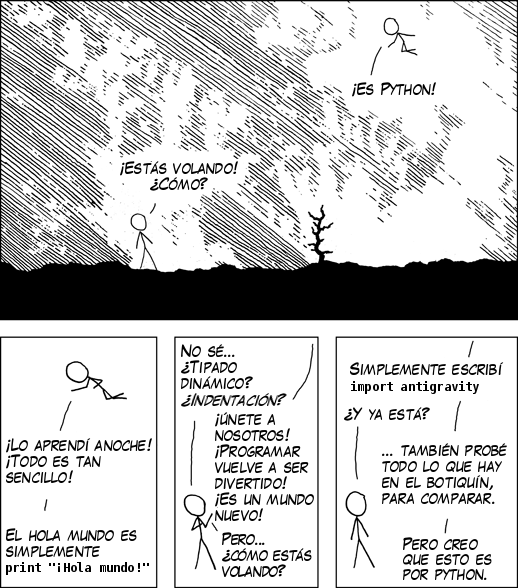
\includegraphics[scale=0.7]{imgs/python.png}
  \\\textit{Figura 1: Python siendo mayormente usado como lenguaje de programación, siendo un lenguaje mayormente interpretado}\\
\end{center}
En algunos casos el uso de lenguajes que son interpretados, generan un consumo significativo de energía y esto en volumenes enormes de información genera problemas en la industria e incluso en las pruebas de performance.
\begin{center}
  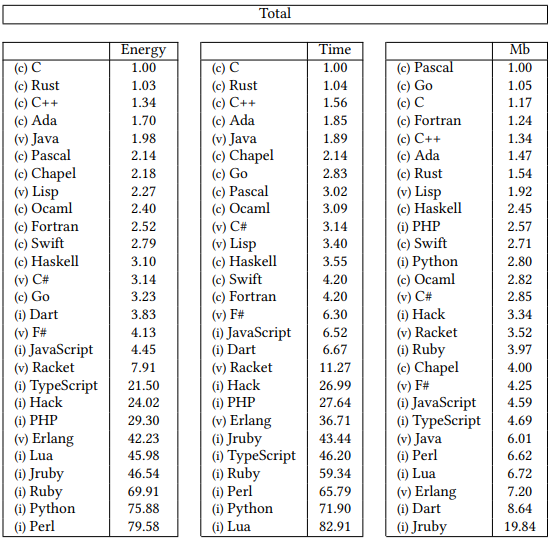
\includegraphics[scale=0.7]{imgs/tabla2.png}
  \\\textit{Figura 2: Tabla de resultados de uso de energía, tiempo y peso en disco de cada lenguaje de programación a los que se realizaron pruebas }\\{\scriptsize Documento de: How Do Energy, Time, and Memory Relate?}
\end{center}
\subsection{Descripción del proyecto}
El compilador realizara uso de modulos de herramientas que nos puede proporcionar el software especializado para la creación y descripción de compiladores, en los cuales se buscara realizar una aproximación de que el compilador y el uso de memoria no cree un consumo excedente de energía, memoria o tiempo al generar el código objeto.
\subsection{Funciones principales}
El compilador es realizado con el fin de poder tener una mejor cercanía con usuarios principiantes los cuales tiene noción de algunos lenguajes de programación como son $Python$, $Ruby$, $Perl$, $etc$.\\Si bien estos lenguajes son considerados lenguajes de alto nivel, se pretende realizar un compilador que realice algunas  operaciones en las que puedan tener un acercamiento a estos tipos de lenguajes y que más tarde puedan mudar de un lenguaje a otro.
\subsection{Justificación}
El proyecto a desarrollar contiene algunos puntos a resaltar de los cuales son Hardware y Software en el que se realizara el desarrollo del producto y de su documentación.
\subsubsection{Hardware}
\begin{itemize}
  \item El hardware en el que sera desarrollado el proyecto trajara bajo una arquitectura x86\_64, debido a que es el actual estandar de desarrollo.
  \item El equipo deseablemente contara con al menos 4GB de RAM.
  \item Procesador dualcore o más cores superior a 1GHz.
\end{itemize}
\subsubsection{Software}
\begin{itemize}
  \item El producto pretende crear un pseudolenguaje que se compila y pretende tener una mejor cercanía con el programador principiante.
  \item El Sistema Operativo en el que se desarrollara y sera la plataforma en la que se ejecutara el proyecto sera en sistema Linux, debido a que las herramientas de trabajo como el analizador léxico, sintactico y semantico pueden encontrarse en paqueterias libres que proporciona Linux.
  \item Se pretende hacer uso de herramientas que proporciona la terminal como el uso de alias y simbolic links para que las llamadas del compilador sean más sencillas en su uso.
  \item Tambien se en la instalación de la paqueteria del compilador se añadiran los manuales pertinentes para que el usuario pueda trabajar correctamente con el producto.
\end{itemize}

\subsection{Innovación}
La innovación del producto de software es el hacer uso de estandares que nos pueden proporcionar el estandar de POSIX, y algunas otras buenas practicas de la programación de modulos de software.\\
Por otro lado tambien es necesario el hacer uso de algoritmos que permitan optimizar el uso de energía que genera la creación y ejecución de código en su entorno de programación.\\
Por lo tanto, si bien es un tiempo corto para la realización de todas las actualizaciones y desarrollo, es bueno planificar el hecho de que pueda existir una aproximación a prototipos del compilador.
\subsection{Complejidad}
De acuerdo a la idea de proyecto a realizar es una tarea larga ya que requiere no solo de uso de herramientas que puede ofrecer el proyecto de GNU/Linux sino que tambien implica el aprendizaje de las mismas y por otro lado tambien implical el uso de herramientas que permitan realizar pruebas de estres y testing como puede realizarlo algunas herramientas de scripting como lo son $Bash$, $sh$, $Ruby$, $Python$.
\subsection{Paradigma de desarrollo}
El paradigma a utilizar para el proyecto sera el uso de prototipos, así como en la escritura de código sera en el paradigma Estructurado ya que este nos permitira trabajar con las herramientas que nos ofrece el Sistema Operativo, y un poco de paradigma Orientado a Objetos para hacer uso de algunas herramientas que nos ofrece el mismo, como la modularidad y el uso de algunos empaquetamientos.
\subsection{Tecnicas de desarrollo}
Para la recolección de requisitos se llevara acabo una encuesta en la cual nos permitira recabar información, en la cual podremos interpretar la dirección final y los detalles a pulir del proyecto, en los cuales podremos saber si los encuestados tienen una facilidad o dificultad a la hora de trabajar con un lenguaje de programación compilado.\\
Los hitos planificados del proyecto es trabjarlo con base en el modelo de prototipos para despúes poder refinar los hitos consiguientes, debido a que es un modelo más sencillos para la realización del producto.\\
Tambien se planea el uso de paradigmas como el orientado a objetos y el estructurado para el desarrollo de los modulos/prototipos.
\printindex

\end{document}
